\subsection{Terrain Generation}

Generation of the underlying terrain is managed by the TerrainGenerator function (see Table \ref{table:terrgen}).
In this implementation, the terrain is represented as a colored and textured surface mesh with evenly spaced vertices, whose heights (y-position) have been altered to form hills and valleys.
The vertices of the mesh are given different height values based on a layered Simplex noise, whose implementation was extracted into a separate module as it would come to use in Population Generation as well.

\begin{table}[H]
  \centering
  \begin{tabular}{lllll}
    \textbf{Input} & & \textbf{Function} & & \textbf{Output} \\
    \midrule
    \textit{Size, Offset, SeaLevel} & $\rightarrow$ & \textbf{TerrainGenerator} & $\rightarrow$ & \textit{Terrain} \\
    \bottomrule
  \end{tabular}

  \caption{Definition of the TerrainGenerator function which is responsible for generating the terrain.}
  \label{table:terrgen}
\end{table}
\vspace{-0.4cm} % Mimic spacing below figures

The input of this function is a set of scalars, specified by the user at runtime.
\textit{Size} determines the width (x-axis) and depth (z-axis) of the terrain,
\textit{Offset} affects the sampling location of the noise, and \textit{SeaLevel} configures the y-position of the surrounding sea, which is represented as a flat, textured plane.
The intention behind \textit{Offset} was to give the user finer control over the noise (and thus the heights) of the terrain.

The noise function used for the terrain had four manually designed noise layers, which intended to form a balanced variation of lakes, plains, and mountains.
The resulting mesh would then be textured and colored in order to make it look more convincing (see Figure \ref{fig:terrcomp}).
Colors were applied based on height levels, forming a blend between snowy mountain tops and verdant plains.
To texture the mesh, a single texture was used with randomized UV coordinates, which was included to reduce Moiré patterns \cite{moire_pattern}.
A texture atlas could have been used to support more textures, but the visuals from this approach were satisfactory enough.

\begin{figure}[h!]
  \centering
   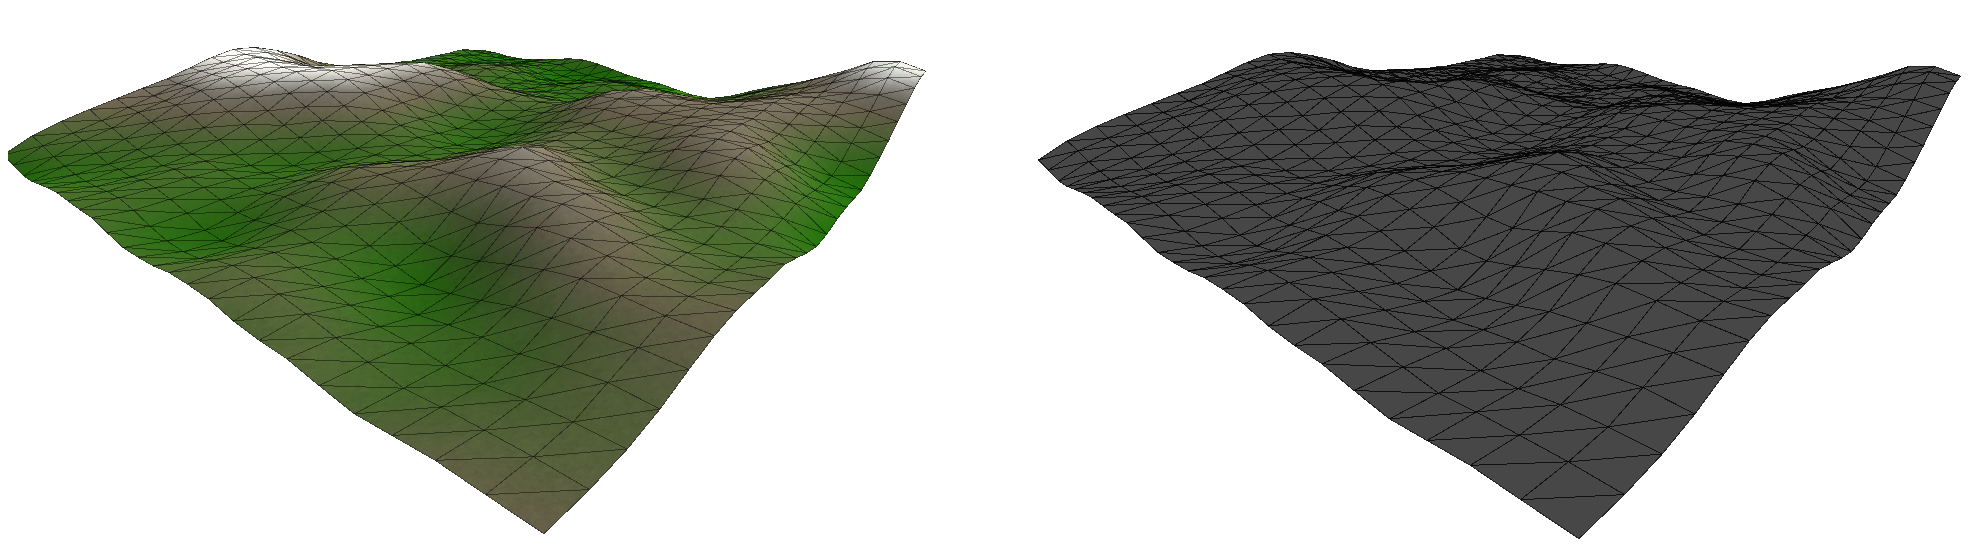
\includegraphics[width=\textwidth]{figure/terraincomparison.png}
   \caption{Example of a surface mesh with (left) and without (right) textures.}
  \label{fig:terrcomp}
\end{figure}

There were two options considered regarding the construction of the terrain.
The first option was to make use of Unity's built-in terrain API, and the second was to construct a custom mesh, manipulating vertex data manually.
The former option showed greater potential as it provided several advanced features such as texture splatting and dynamic resolution.

Unfortunately, these features were only applicable in runtime and could not be serialized into model files in any simple way.
Furthermore, the produced terrains were custom objects specific to Unity, and would have to be converted into meshes before exportation.
Thus, the second option was chosen as it would provide a simpler implementation.
